%% This is file `elsarticle-template-1-num.tex',
%%
%% Copyright 2009 Elsevier Ltd
%%
%% This file is part of the 'Elsarticle Bundle'.
%% ---------------------------------------------
%%
%% It may be distributed under the conditions of the LaTeX Project Public
%% License, either version 1.2 of this license or (at your option) any
%% later version.  The latest version of this license is in
%%    http://www.latex-project.org/lppl.txt
%% and version 1.2 or later is part of all distributions of LaTeX
%% version 1999/12/01 or later.
%%
%% The list of all files belonging to the 'Elsarticle Bundle' is
%% given in the file `manifest.txt'.
%%
%% Template article for Elsevier's document class `elsarticle'
%% with numbered style bibliographic references
%%
%% $Id: elsarticle-template-1-num.tex 149 2009-10-08 05:01:15Z rishi $
%% $URL: http://lenova.river-valley.com/svn/elsbst/trunk/elsarticle-template-1-num.tex $
%%
% \documentclass[preprint,12pt]{elsarticle}

%% Use the option review to obtain double line spacing
%% \documentclass[preprint,review,12pt]{elsarticle}

%% Use the options 1p,twocolumn; 3p; 3p,twocolumn; 5p; or 5p,twocolumn
%% for a journal layout:
% \documentclass[final,1p,times]{elsarticle}
\documentclass[10pt,final,1p,times,twocolumn]{elsarticle}
%% \documentclass[final,3p,times]{elsarticle}
%% \documentclass[final,3p,times,twocolumn]{elsarticle}
%% \documentclass[final,5p,times]{elsarticle}
%% \documentclass[final,5p,times,twocolumn]{elsarticle}

%% if you use PostScript figures in your article
%% use the graphics package for simple commands
%% \usepackage{graphics}
%% or use the graphicx package for more complicated commands
%% \usepackage{graphicx}
%% or use the epsfig package if you prefer to use the old commands
%% \usepackage{epsfig}

%% The amssymb package provides various useful mathematical symbols
\usepackage{amssymb}
\usepackage{multicol}
\usepackage{lipsum}
\usepackage{caption}
\captionsetup[figure]{font=large,labelfont=large}
\captionsetup[table]{font=large,labelfont=large}
%% The amsthm package provides extended theorem environments
%% \usepackage{amsthm}

%% The lineno packages adds line numbers. Start line numbering with
%% \begin{linenumbers}, end it with \end{linenumbers}. Or switch it on
%% for the whole article with \linenumbers after \end{frontmatter}.
% \usepackage{lineno}

%% natbib.sty is loaded by default. However, natbib options can be
%% provided with \biboptions{...} command. Following options are
%% valid:

%%   round  -  round parentheses are used (default)
%%   square -  square brackets are used   [option]
%%   curly  -  curly braces are used      {option}
%%   angle  -  angle brackets are used    <option>
%%   semicolon  -  multiple citations separated by semi-colon
%%   colon  - same as semicolon, an earlier confusion
%%   comma  -  separated by comma
%%   numbers-  selects numerical citations
%%   super  -  numerical citations as superscripts
%%   sort   -  sorts multiple citations according to order in ref. list
%%   sort&compress   -  like sort, but also compresses numerical citations
%%   compress - compresses without sorting
%%
%% \biboptions{comma,round}

% \biboptions{}

\usepackage{amsmath}% http://ctan.org/pkg/amsmath
\newcommand\sufr[3][0pt]{$\rule{0pt}{\dimexpr#1+1.4ex\relax}^\frac{#2}{#3}$}


\usepackage{graphicx}

\usepackage{algorithmic}
\usepackage{algorithm}

\usepackage{subfigure}
\usepackage{stfloats}


\journal{Lancet Digital Health}

\begin{document}

\begin{frontmatter}
\title{DigiOnco: A Pipeline to Unveil Digital Non-Invasive Biomarkers from Multi-parametric Radiomics Footprints}

%% use optional labels to link authors explicitly to addresses:
% \author[label1,label2]{<author name>}
%  \address[label1]{<address>}
%  \address[label2]{<address>}

\author[label1]{Santhi Natarajan, Anand Ravishankar, Bharathi Malakreddy A}
\author[label2]{G.Lohith, Kritika Sekar, Shivakumar Swamy, Kumar Kallur, Basavalinga Ajai Kumar, Mahesh Bandimegal, Krithika Murugan}
\address[label1]{BMS Institute of Technology and Management, Visweswaraiah Technological Univesity, Bangalore, India}
\address[label2]{Health Care Global Hospitals, Bangalore, India}
\end{frontmatter}
\section{Appendix}

\subsection{Data Acquisition}

\subsection{Data Interpretation}

\begin{figure*}[!b]
\centering
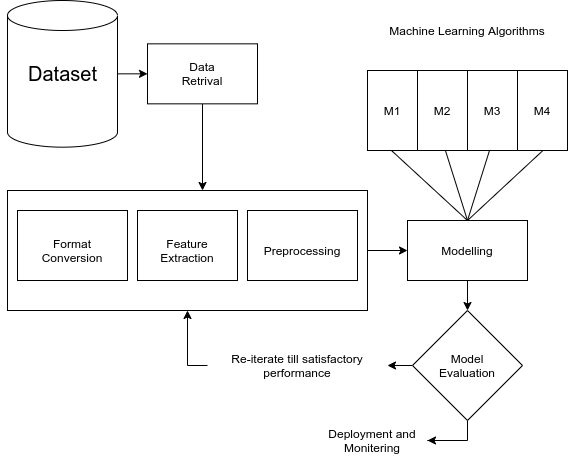
\includegraphics[width=10.7cm]{flowchart.png}
\caption{Flowchart showing the steps involved in obtianing the final results}
\label{img1}
\end{figure*}

Figure $\ref{img1}$ breaks down the data interpretation process into a conglomerate of submodules which function serially to perform the classification task. The images obtained from the previous process are stored in a cataloging structure for easy access. Note that the images are tagged with their target class by a specialist beforehand. The images are converted to a suitable format for feature extraction. The end product is obtained in the form of a structured dataset consisting of the target class and an array of feature-filter mapping. Preprocessing techniques are applied to the normalize the values throughout the dataset and to remove any redundant entries. Principal Component Analysis (PCA) was applied to reduce the feature space whilst witholding components with the highest information content. The dataset is shuffled randomly and split into two categories (training and testing sets) in a ratio of 70:30. Multiple machine learning algorithms are queued onto the training set and the results are tabulated accordingly. The model evaluation process is repeated till either a set number of iterations are completed or till the performance metrics are acceptable. Once the parameters corresponding to the optimal performance are achieved, the test set is re-introduced into the model. Using the tuned parameters, the model makes a prediction on the test set and a score is generated with the test set's inital targets baseline. Provided a sufficient scored is obtained, statistical inferences can be drawn from the testing phase. 

The preceding process is performed for 2 classification tasks: TN vs Non-TN, and HER vs Luminal-A vs TN. Tables $\ref{tab1}$ and $\ref{tab2}$ showcase the optimal feature-filter mapping for both the tasks respectively. Note that this mapping is a subset of the set of features and filters described in the main material.          
% The following material describes the entire result set obtained during the study. To recapitulate, our study consisted of two classification tasks namely, TN vs Non-TN and TN vs Luminal-A vs HER. Once the training phase is completed the model configuration is loaded into the testing mechanism. The test data consisted solely of Luminal-B patients given the correlation of Luminal-A and Luminal-B data characteristics. The results described in the main material concludes at the training phase and provides a taste of the actual digital biomarkers obtained. Tables $\ref{tb1}$ and $\ref{tb2}$ provide a summary of the features selected after the pre-processing step. The selection is done mainly on the amount of distingushing information each feature offers. Moreover, various filters have also been applied to provide a expansive view.  The corresponding box plots having been shown in Figure Sets $\ref{f1}$ and $\ref{f2}$. Notice that not all box plots can be utilized optimally for distinuishing the different classes due to closeness in the measured value. To counter this problem, we introduced the concept of higher dimension plots which provide a user-friendly interface to the end user. A clear correlation can be established between the features and targets resulting in a more informed decision making stance.  

\subsection{Statistical Analysis}

Figures $\ref{1-4}$ to $\ref{t_13-15}$ depict the box and whisker plots obtained for the feature-filter mapping specified respectively. These plots summarize the variability and distribution of the select variable. Note that even though the feature-filter mapping is optimal, the data distribution might be too similar for a naked eye observation to make a clear distinction. Clear examples for this can be found in figures corresponding to entries 3, 11, and 13 in Table $\ref{tb1}$ and entries 1, 4, 5, and 15 in Table $\ref{tab2}$.  

\begin{table}[!b]
\centering
\caption{\textbf{Final Feature-Filter Mapping}: TN vs Non-TN}
\label{tb1}
\begin{tabular}{| c | c | c |}
\hline
\textbf{Sr. No.} & \textbf{Feature} & \textbf{Filter}\\
\hline
1& GLCM\_Cluster\_Shade & LoG\\
\hline
2& GLCM\_Cluster\_Shade & Nil \\
\hline
3& FirstOrder\_Minimum & Square\\
\hline
4& NGTDM\_Coarseness & Square\\
\hline
5& FirstOrder\_Mean & Wavelet = HHH \\
\hline
6& FirstOrder\_Skewness & Wavelet = HHH\\
\hline
7& GLCM\_Correlation & Wavelet = HHH\\
\hline
8& FirstOrder\_Energy & Wavelet = HHL\\
\hline
9& FirstOrder\_Energy & Wavelet = HLH\\
\hline
10& FirstOrder\_Mean & Wavelet = HLH\\
\hline
11& FirstOrder\_Skewness & Wavelet = HLH\\
\hline
12& FirstOrder\_Energy & Wavelet = HLL\\
\hline
13& GLCM\_Cluster\_Shade & Wavelet = LHH\\
\hline
14& FirstOrder\_Energy & Wavelet = LLH\\
\hline
15& FirstOrder\_Skewness & Wavelet = LLH\\
\hline
16& FirstOrder\_Energy & Wavelet = LLL\\
\hline
\end{tabular}
\label{tab1}
\end{table}

\begin{table}[!b]
\centering
\caption{\textbf{Final Feature-Filter Mapping}:HER vs Luminal-A vs TN}
\label{tb2}
\begin{tabular}{| c | c | c |}
\hline
\textbf{Sr. No.} & \textbf{Feature} & \textbf{Filter}\\
\hline
1& FirstOrder\_Kurtosis & Exponential\\
\hline
2& GLCM\_Cluster\_Shade & LoG\\
\hline
3& GLCM\_Cluster\_Shade & Nil \\
\hline
4& GLCM\_Cluster\_Prominence & Square\\
\hline
5& GLCM\_Cluster\_Shade & Square \\
\hline
6& GLCM\_Cluster\_Tendency & Square\\
\hline
7& GLCM\_MCC & Square\\
\hline
8& FirstOrder\_Energy & Wavelet = HHL\\
\hline
9& FirstOrder\_Mean & Wavelet = HHL\\
\hline
10& FirstOrder\_Energy & Wavelet = HLL\\
\hline
11& FirstOrder\_Skewness & Wavelet = HLL\\
\hline
12& FirstOrder\_Energy & Wavelet = LHH\\
\hline
13& FirstOrder\_Energy & Wavelet = LHL\\
\hline
14& FirstOrder\_Skewness & Wavelet = LLH\\
\hline
15& GLCM\_Cluster\_Prominence & Wavelet = LLH\\
\hline
\end{tabular}
\label{tab2}
\end{table}

\begin{figure}[hbt!]
\centering
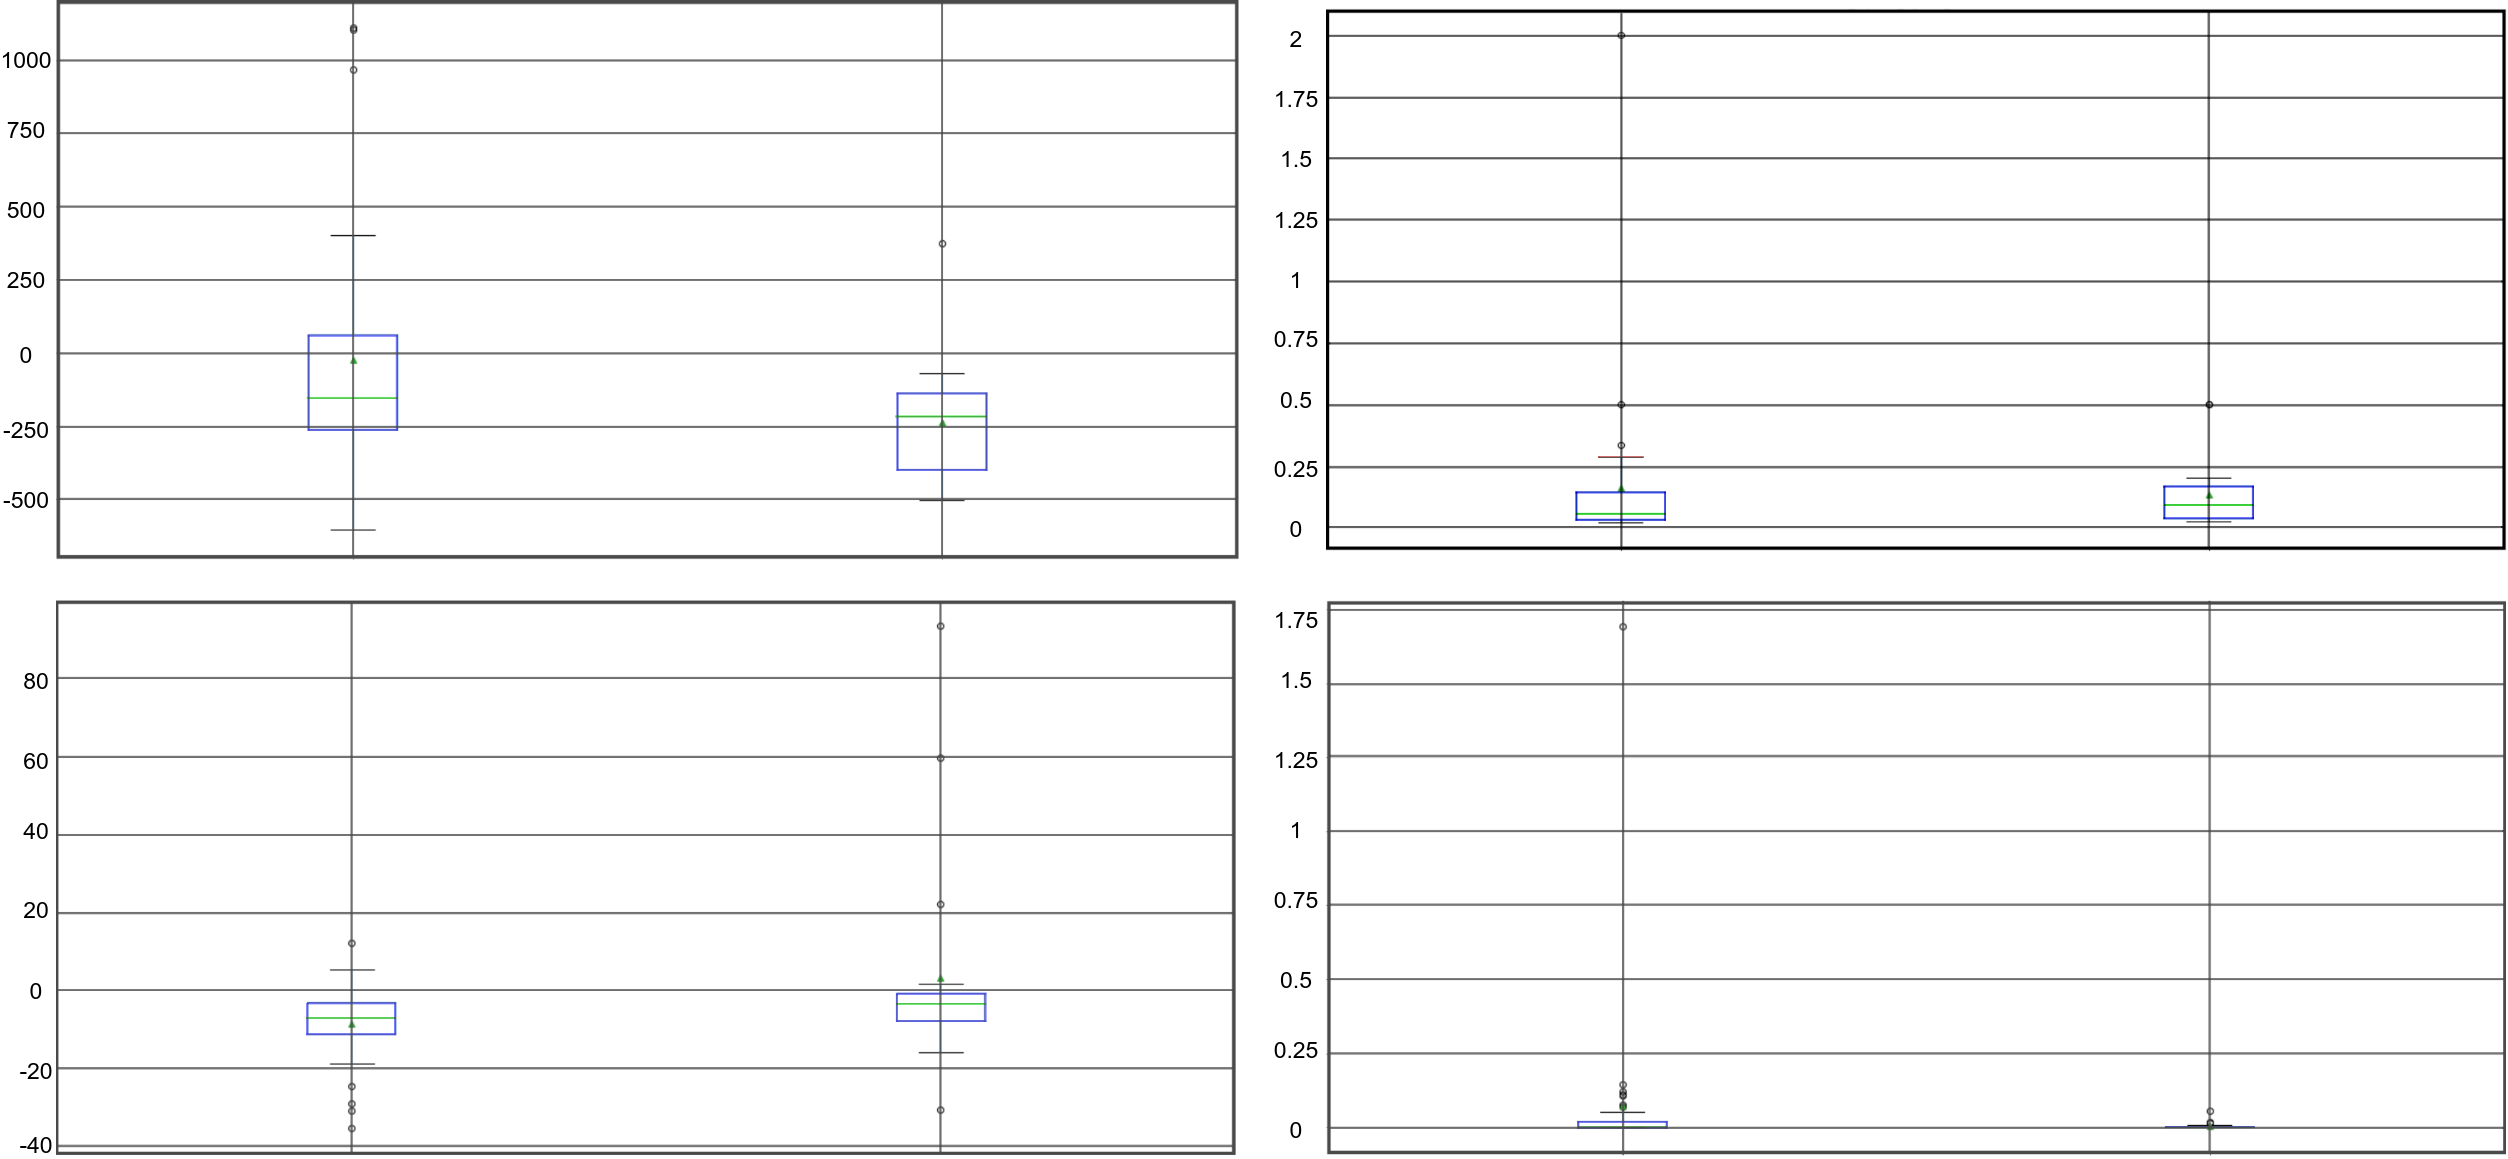
\includegraphics[width=14cm]{1-4.png}
\caption{From top left, counter-clockwise, entries 1-4 of Table $\ref{tab1}$ depicting the distribution of select feature-filter mapping for TN (left) vs Non-TN (right)}
\label{1-4}
\end{figure}
\begin{figure}[hbt!]
\centering
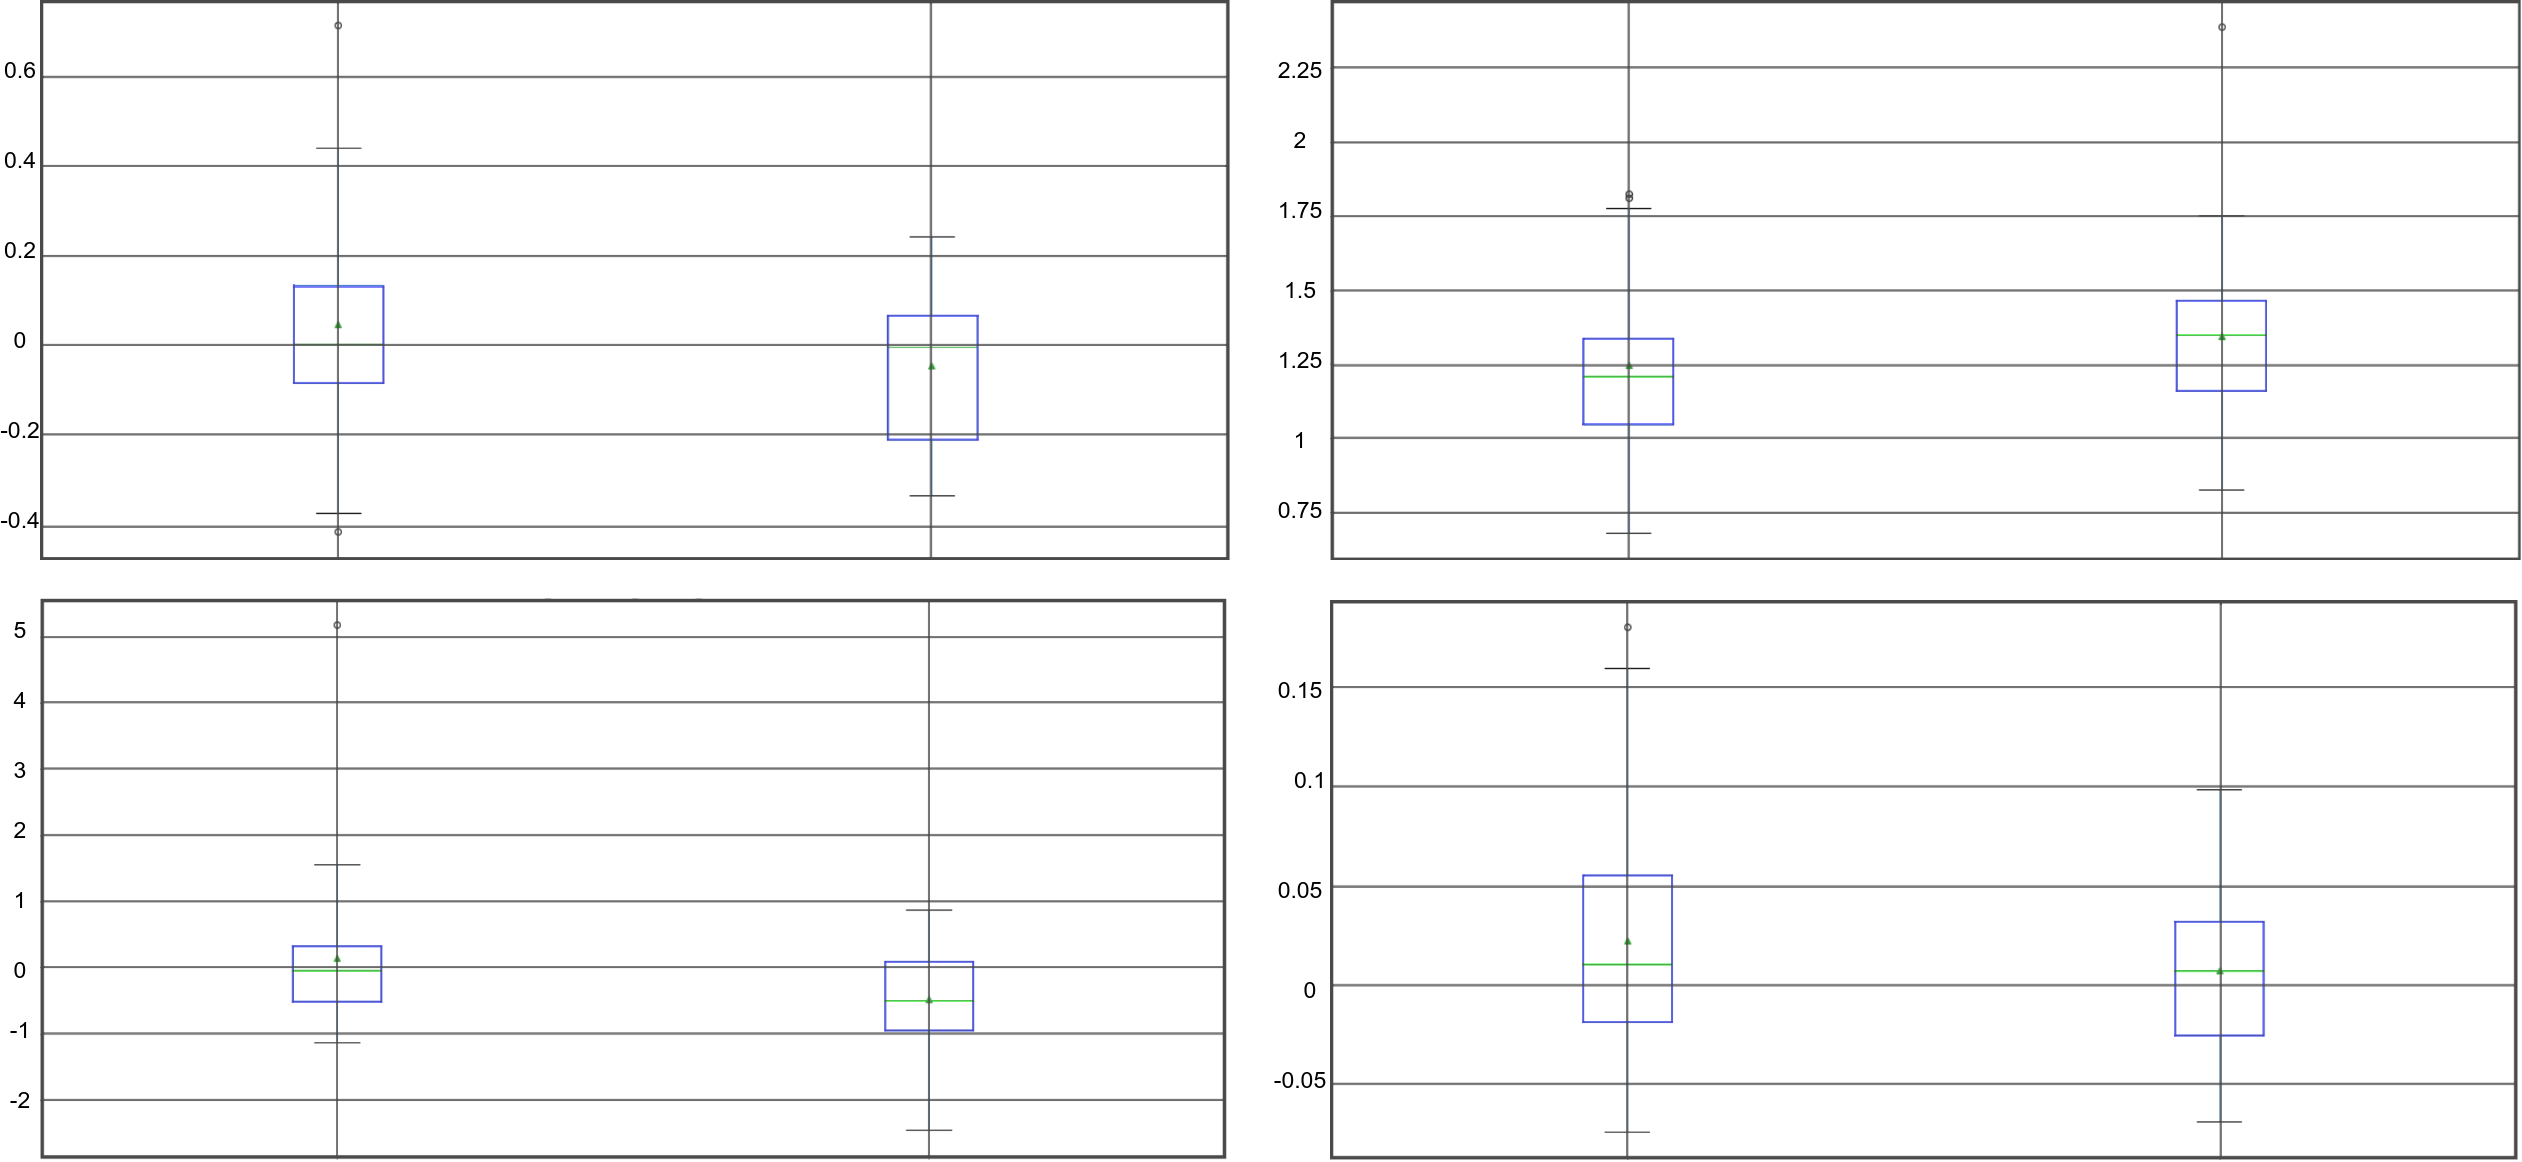
\includegraphics[width=14cm]{5-8.png}
\caption{From top left, counter-clockwise, entries 5-8 of Table $\ref{tab1}$ depicting the distribution of select feature-filter mapping for TN (left) vs Non-TN (right)}
\label{5-8}
\end{figure}
\begin{figure}[hbt!]
\centering
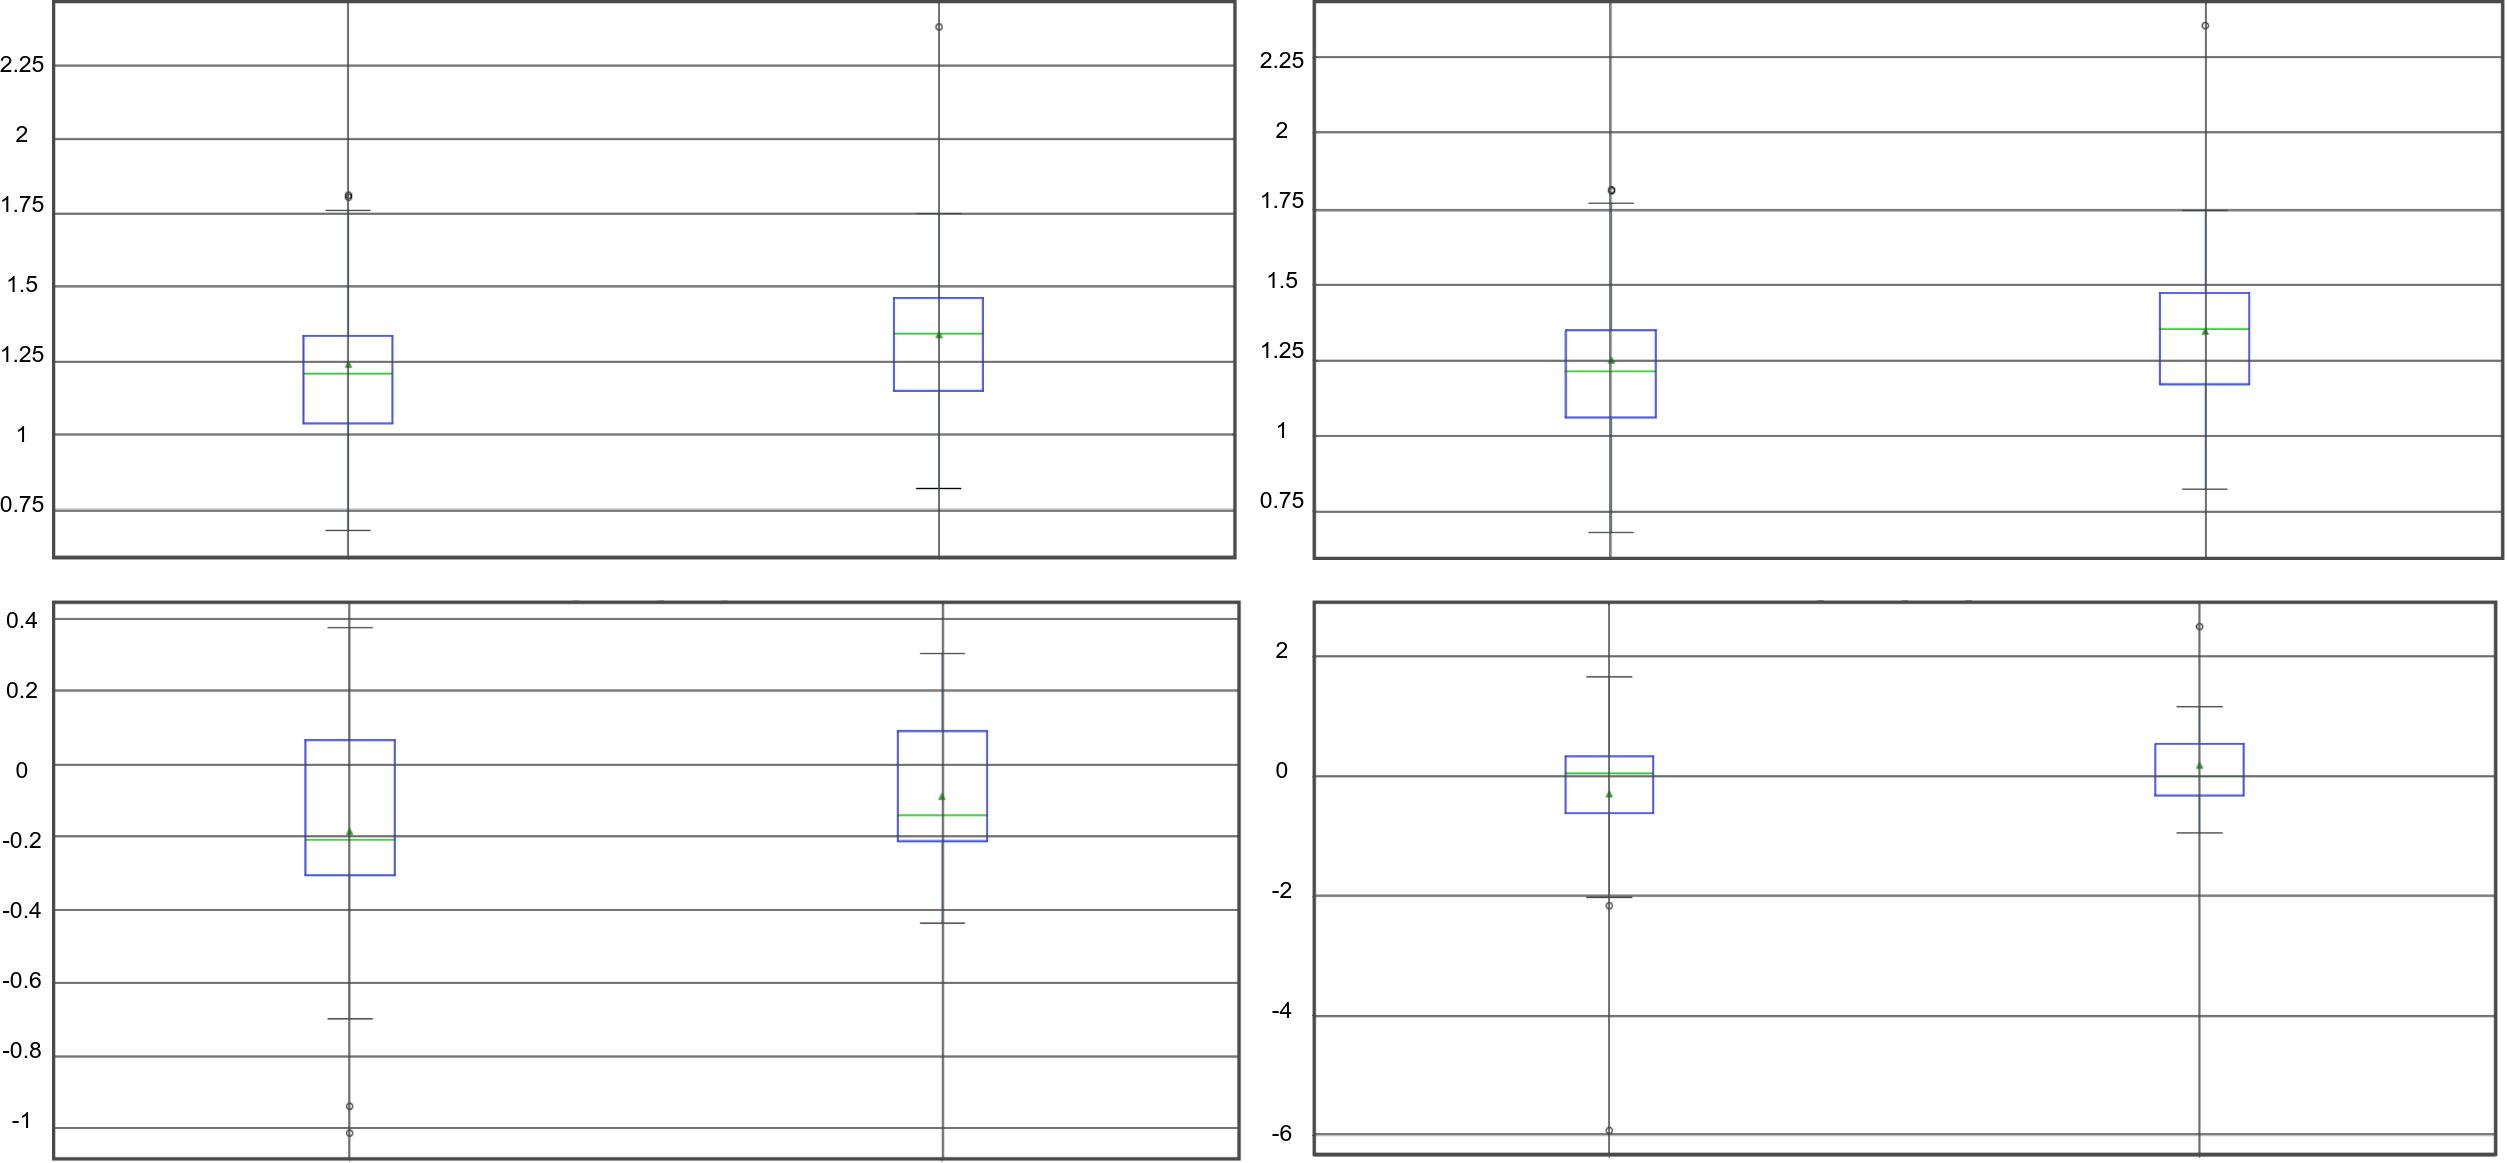
\includegraphics[width=14cm]{9-12.png}
\caption{From top left, counter-clockwise, entries 9-12 of Table $\ref{tab1}$ depicting the distribution of select feature-filter mapping for TN (left) vs Non-TN (right)}
\label{9-12}
\end{figure}
\begin{figure}[hbt!]
\centering
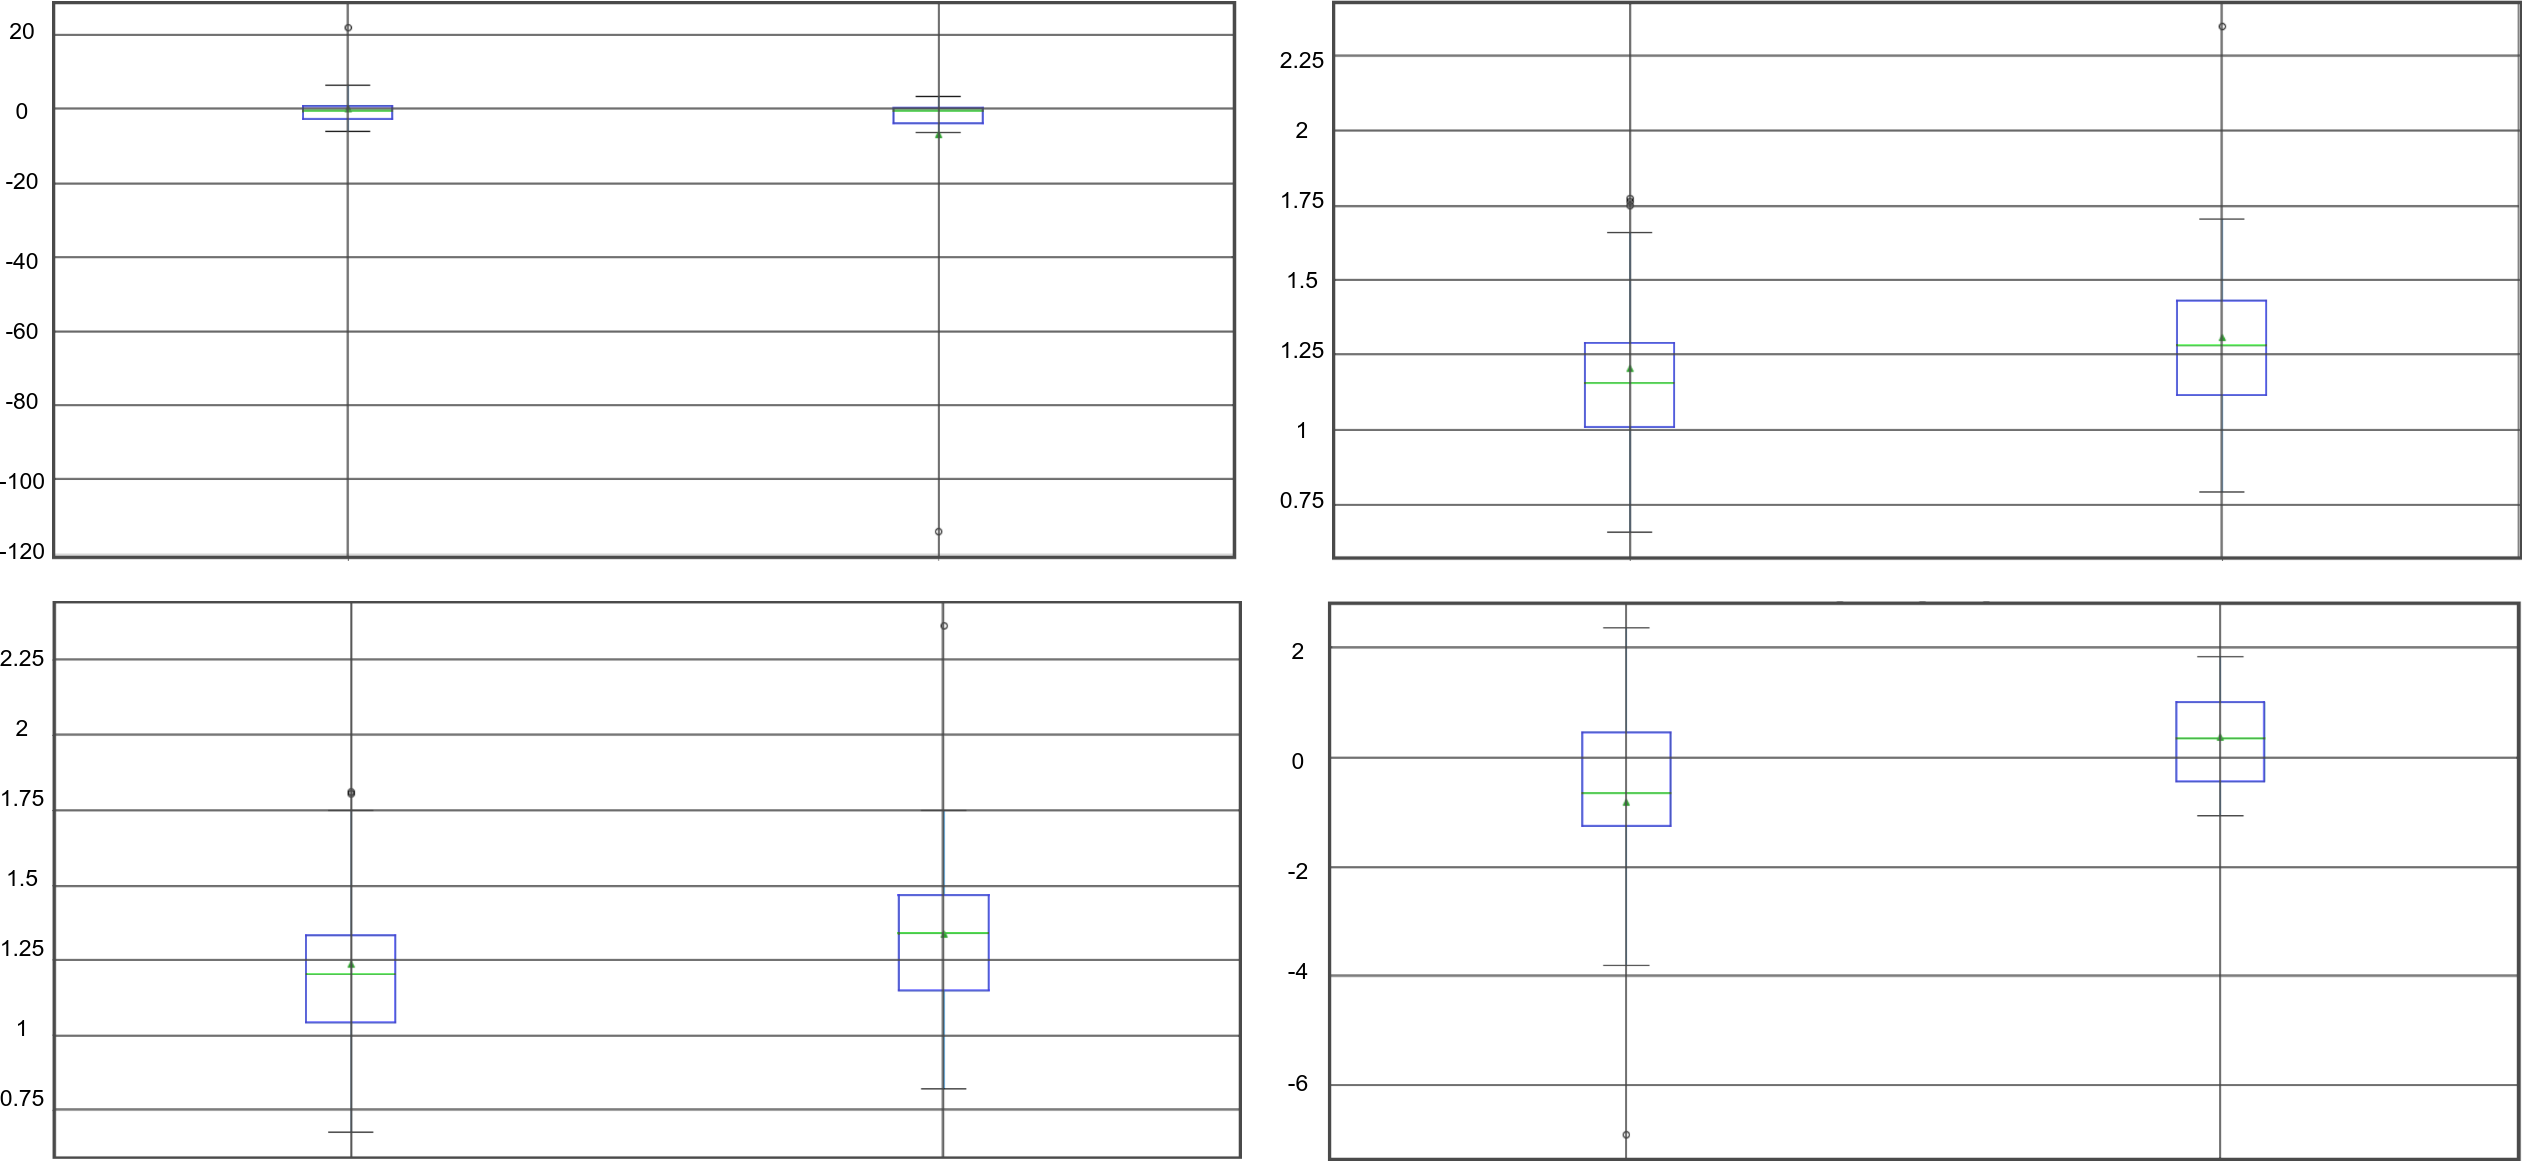
\includegraphics[width=14cm]{13-16.png}
\caption{From top left, counter-clockwise, entries 13-16 of Table $\ref{tab1}$ depicting the distribution of select feature-filter mapping for TN (left) vs Non-TN (right)}
\label{13-16}
\end{figure}

\begin{figure}[hbt!]
\centering
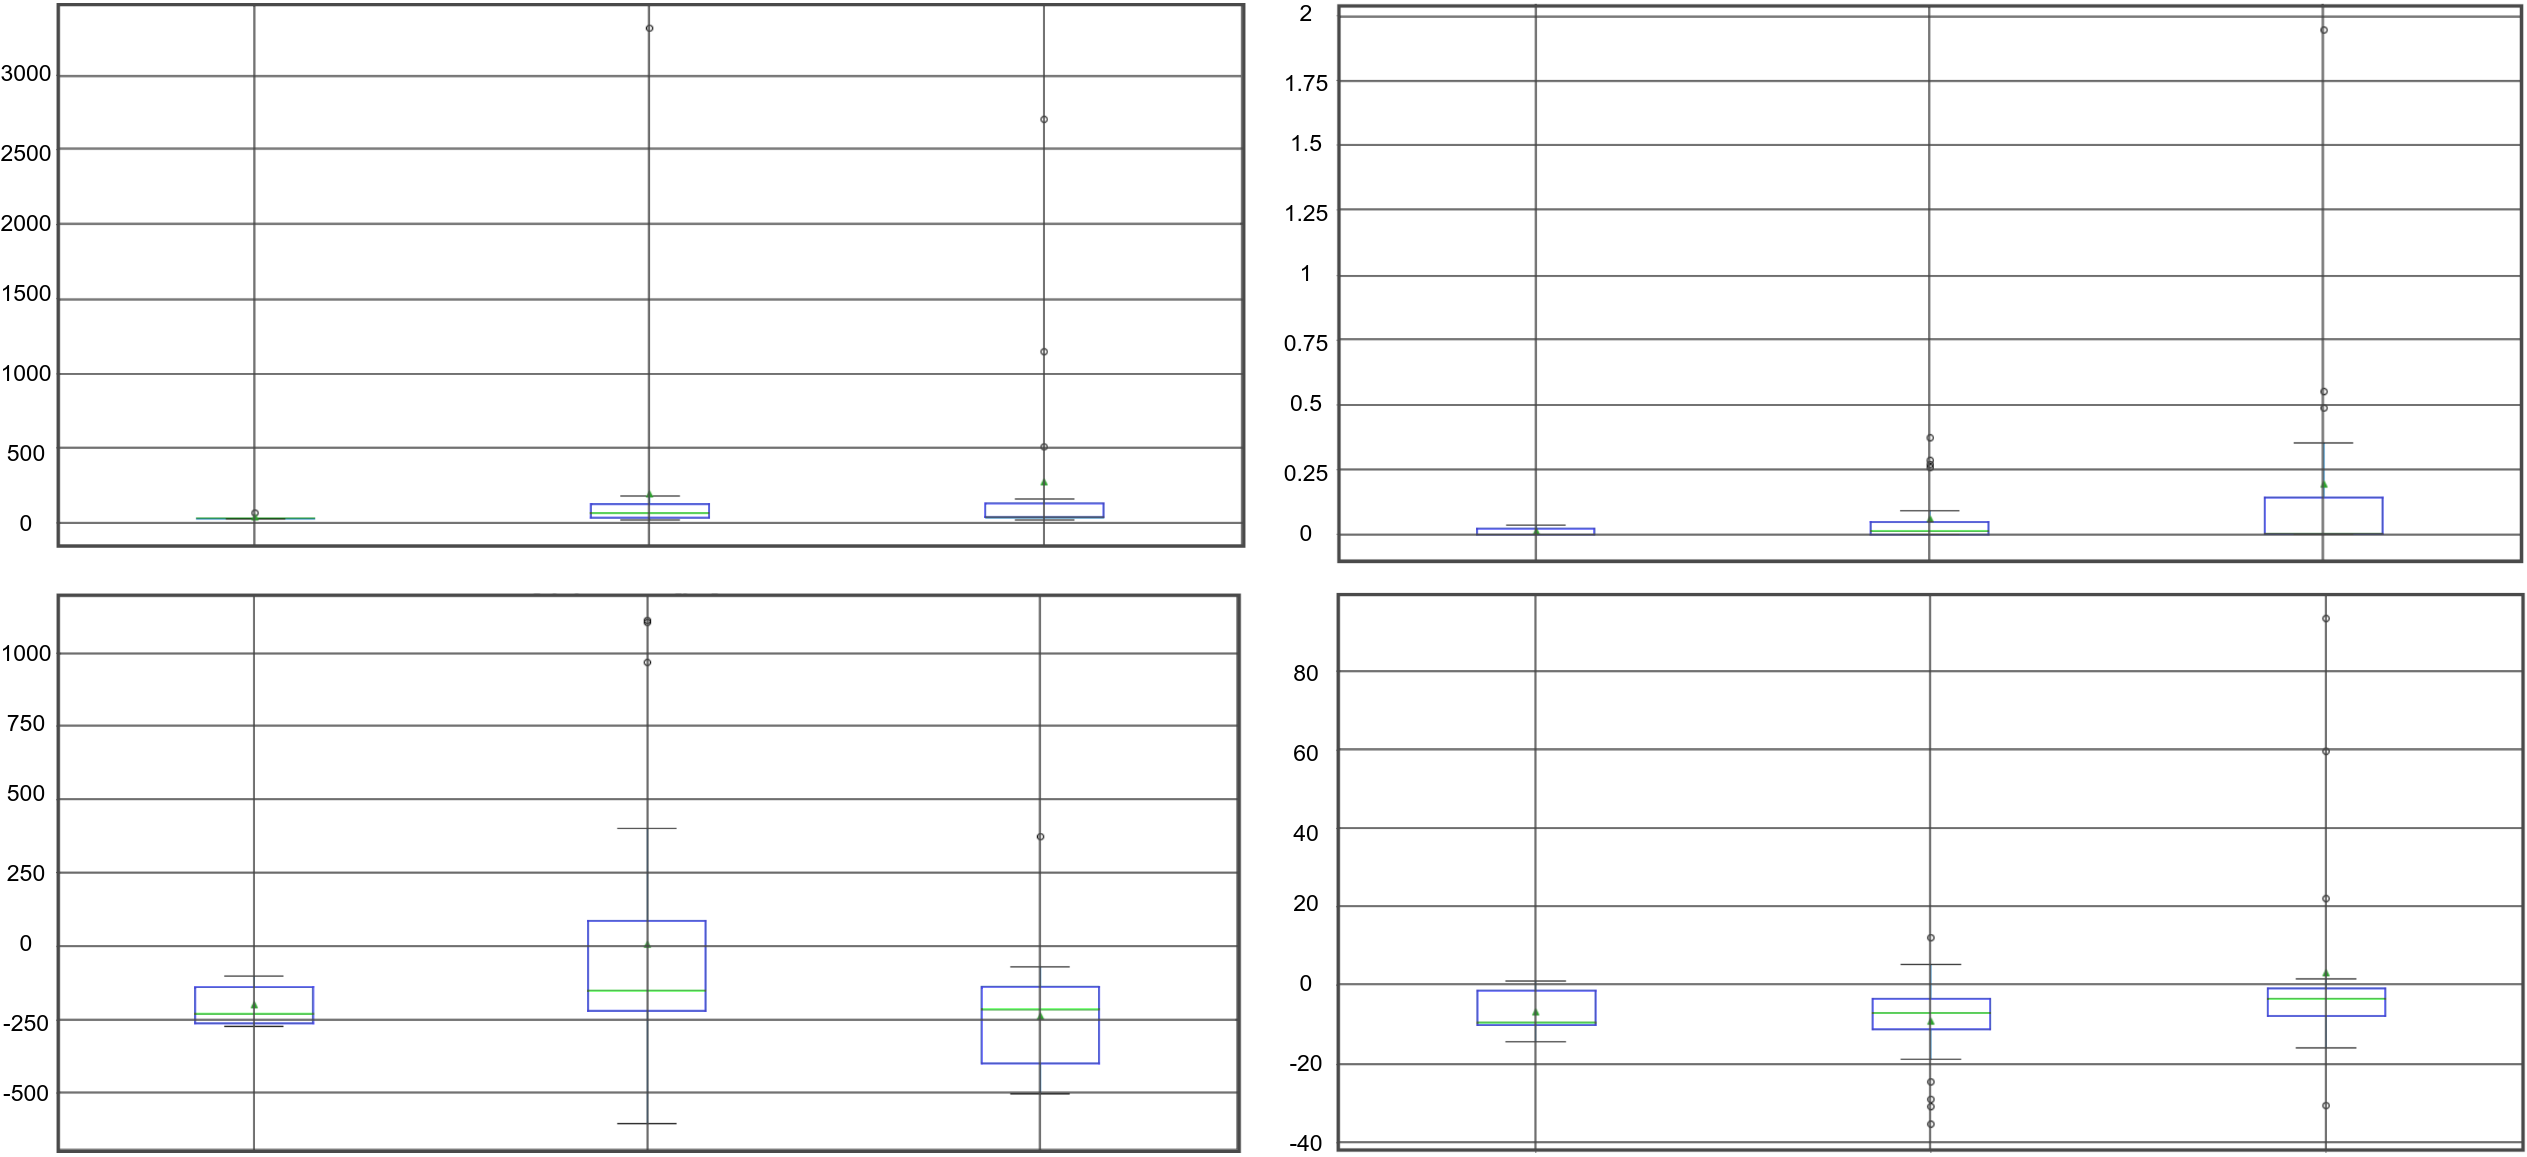
\includegraphics[width=14cm]{t_1-4.png}
\caption{From top left, counter-clockwise, entries 1-4 of Table $\ref{tab2}$ depicting the distribution of select feature-filter mapping for HER (left) vs Luminal-A (center) vs TN (right)}
\label{t_1-4}
\end{figure}
\begin{figure}[hbt!]
\centering
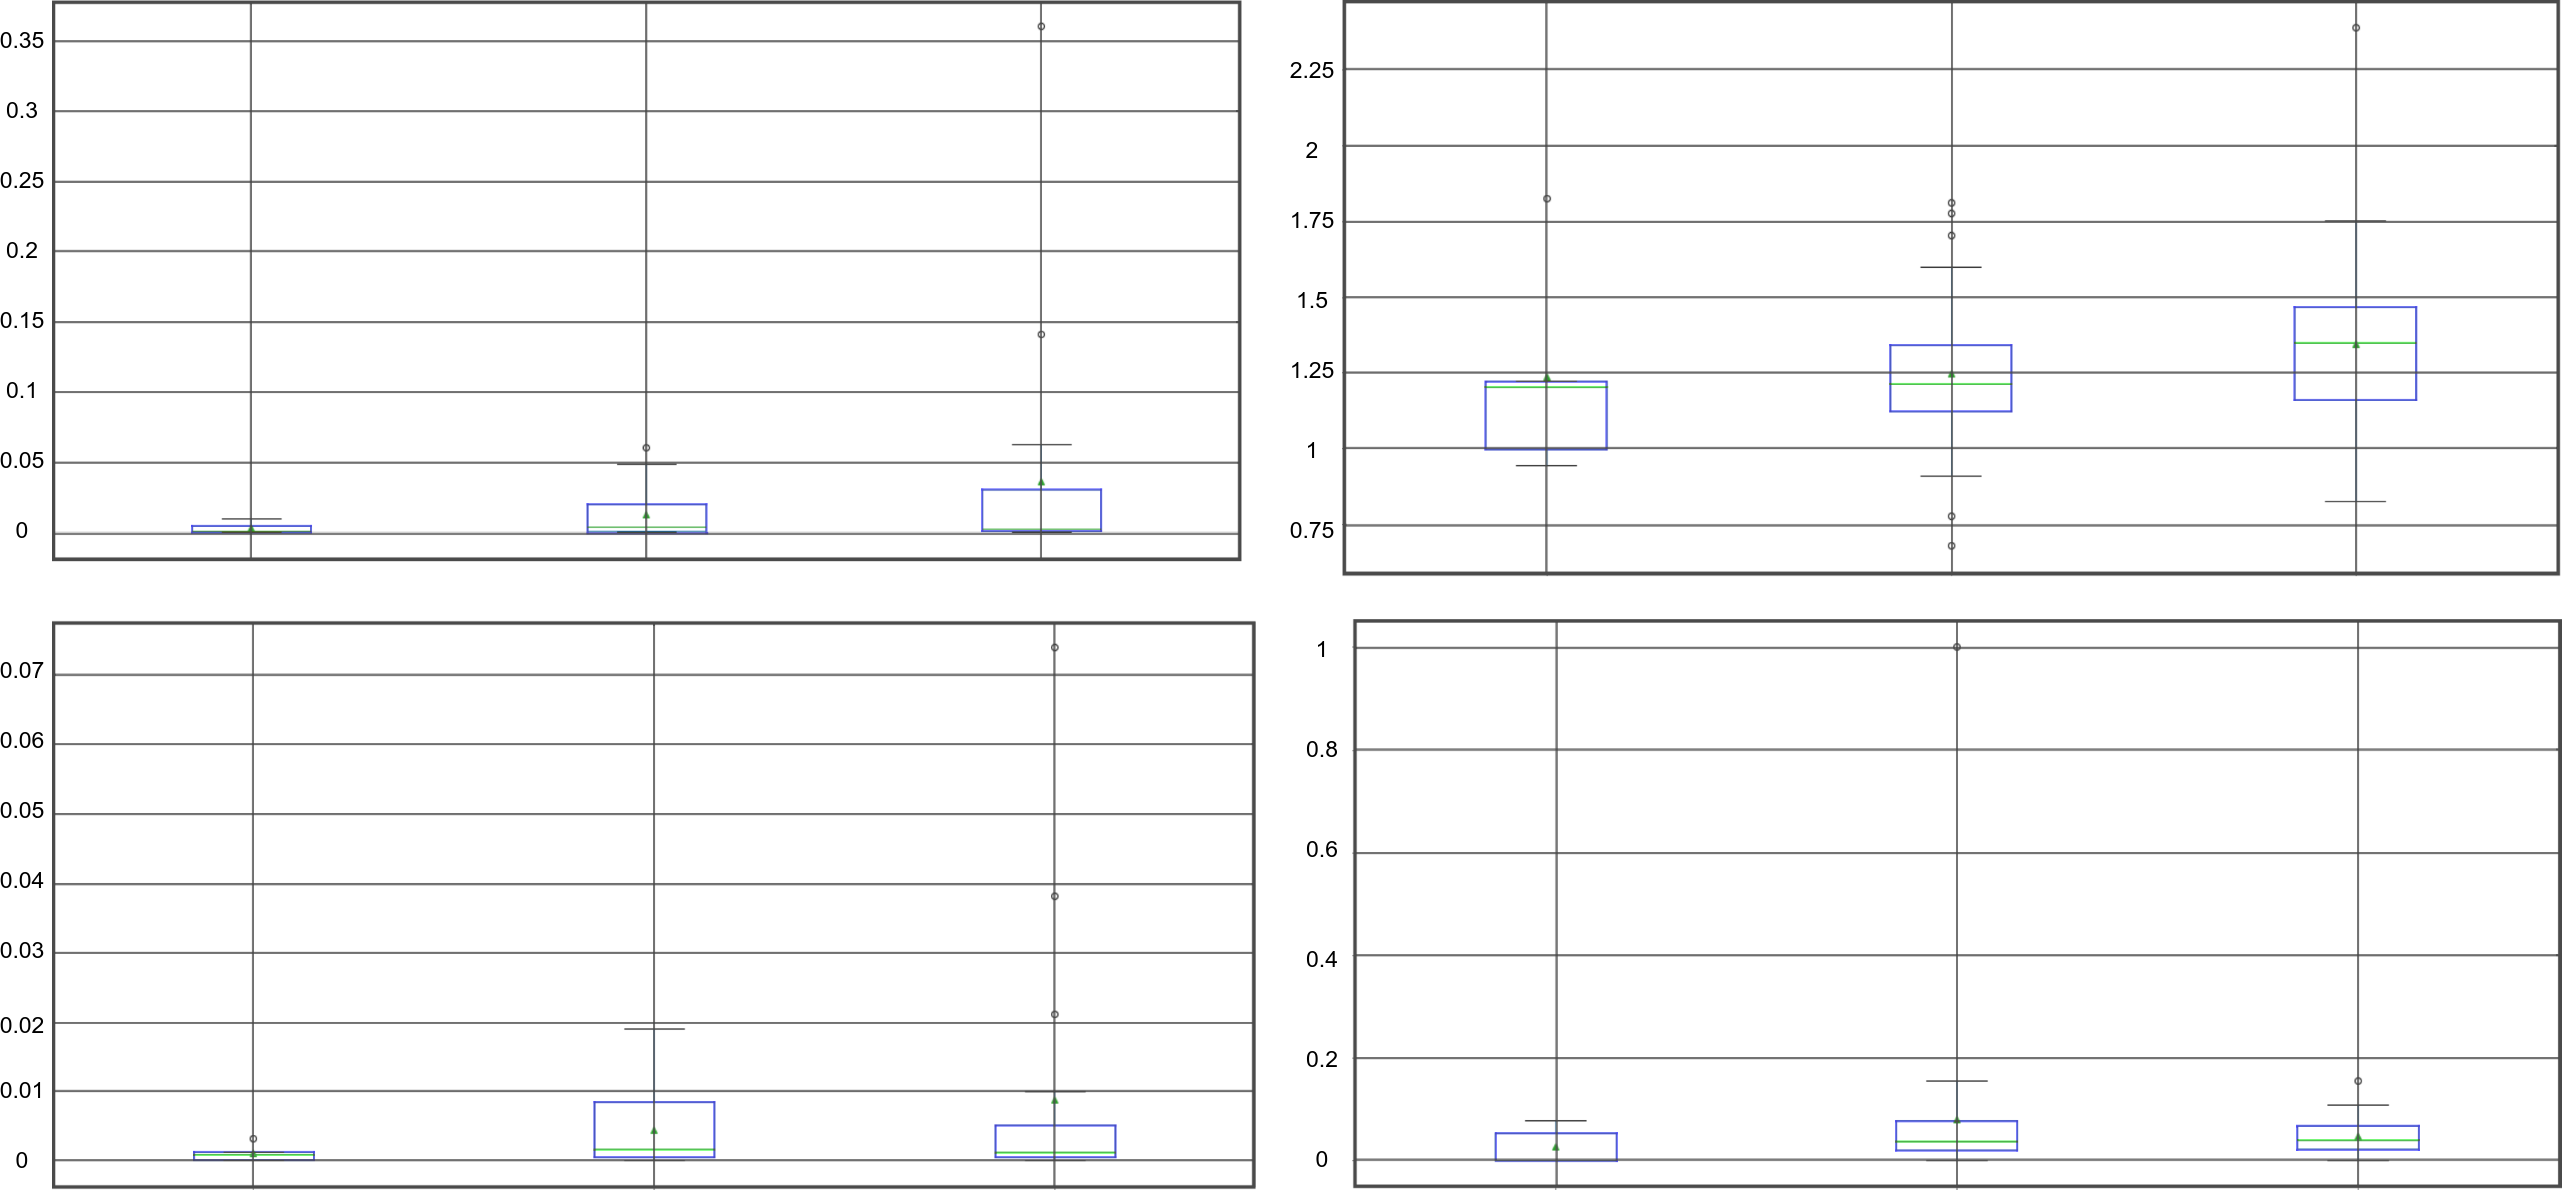
\includegraphics[width=14cm]{t_5-8.png}
\caption{From top left, counter-clockwise, entries 5-8 of Table $\ref{tab1}$ depicting the distribution of select feature-filter mapping for HER (left) vs Luminal-A (center) vs TN (right)}
\label{t_5-8}
\end{figure}
\begin{figure}[hbt!]
\centering
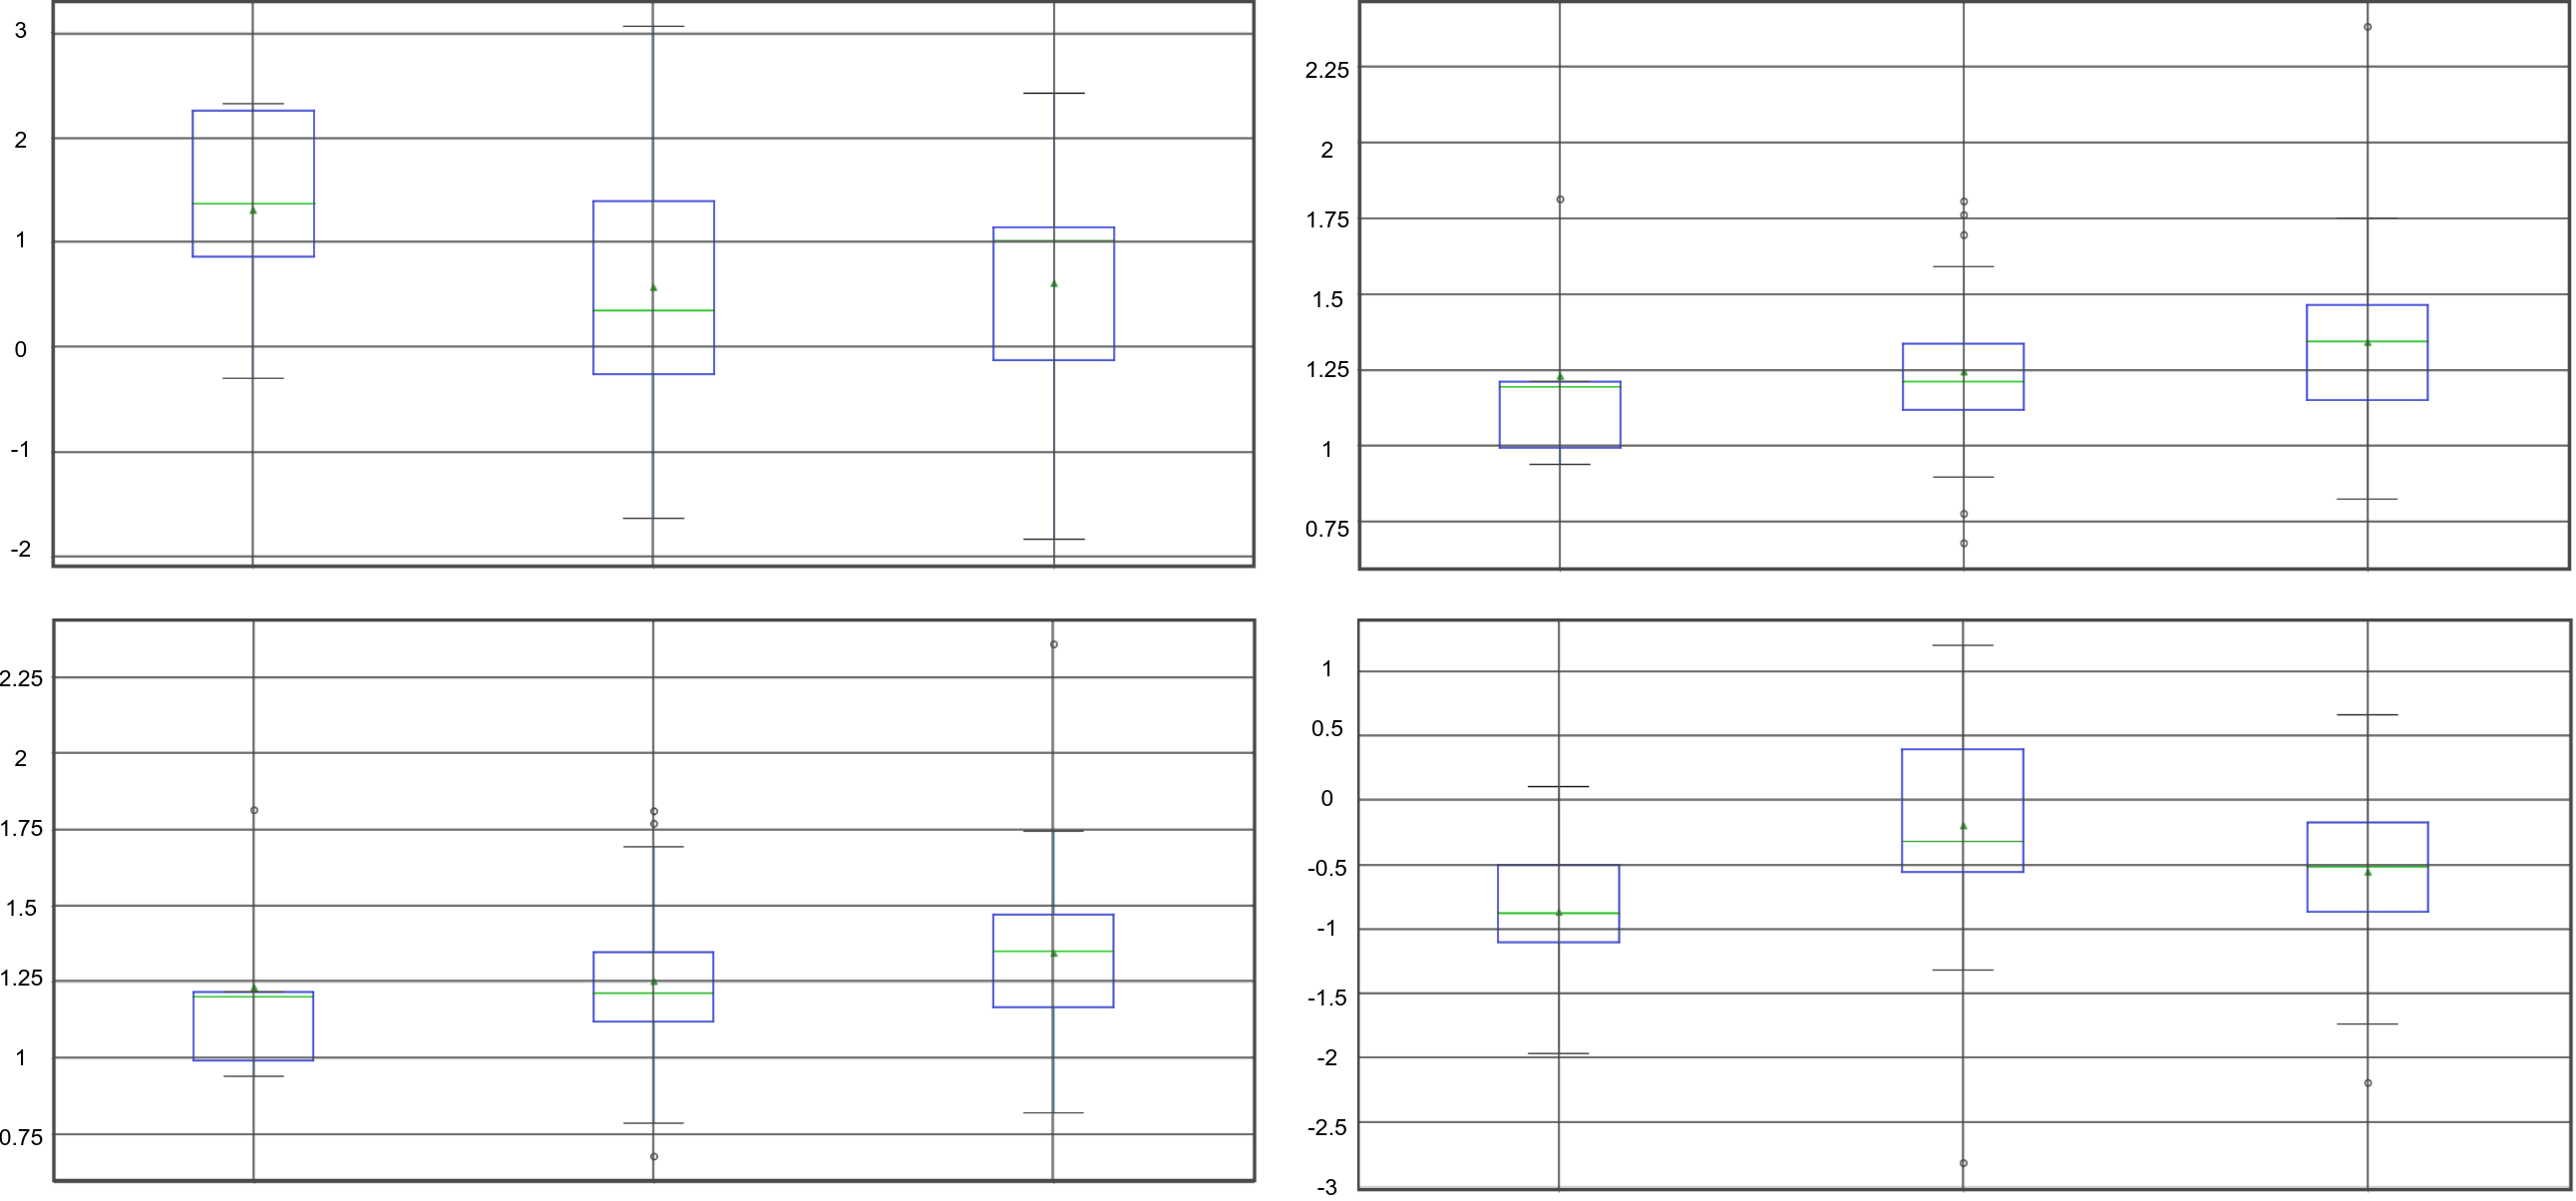
\includegraphics[width=14cm]{t_9-12.png}
\caption{From top left, counter-clockwise, entries 9-12 of Table $\ref{tab1}$ depicting the distribution of select feature-filter mapping for HER (left) vs Luminal-A (center) vs TN (right)}
\label{t_9-12}
\end{figure}
\begin{figure}[hbt!]
\centering
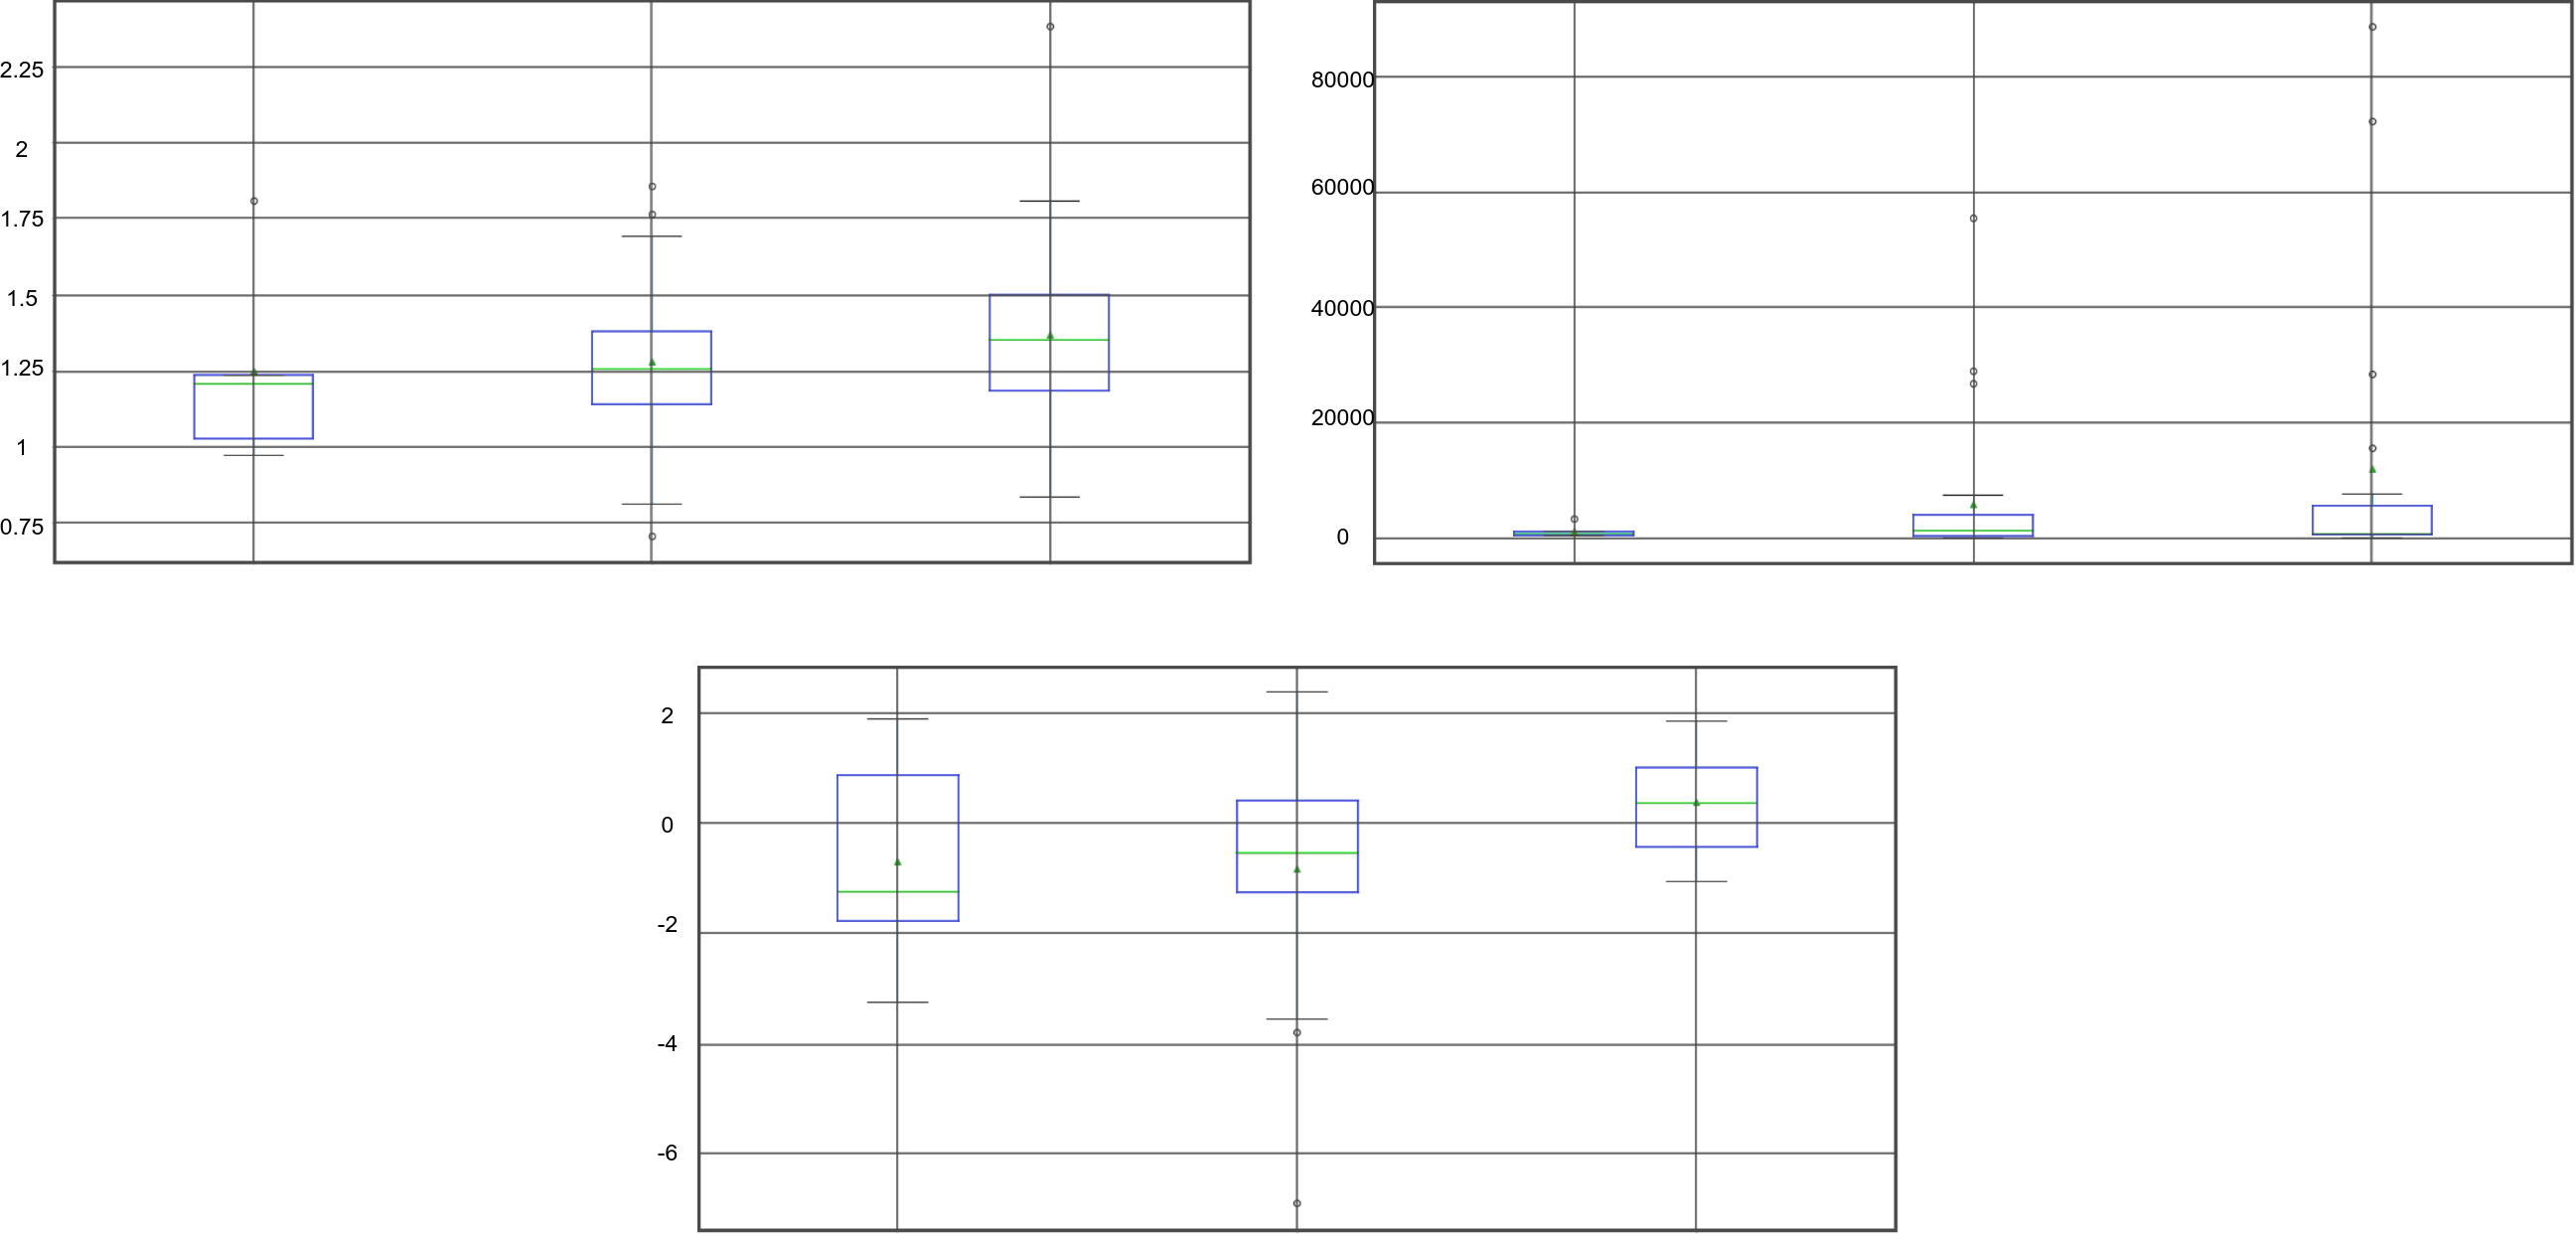
\includegraphics[width=14cm]{t_13-15.png}
\caption{From top left, counter-clockwise, entries 13-15 of Table $\ref{tab1}$ depicting the distribution of select feature-filter mapping for HER (left) vs Luminal-A (center) vs TN (right)}
\label{t_13-15}
\end{figure}

\section{Algorithms Employed}

The data is classified based the features which contrast the classes with the highest information content. The process of data classification using Random Forest is shown in Algorithm $\ref{alg:rf}$. AdaBoost solves the problem of overfitting by presenting the system with the misclassified data and forcing it to improve the overall performance. The two flavours of AdaBoost i.e, SAMME and SAMME.R have been descibed in Algorithms $\ref{alg:samme}$ and $\ref{alg:sammer}$. SFORCE combines the strength of Random Forests and takes care of the  drawbacks by using a Boosting algorithm to make the search process more concentrated as shown in Algorithm $\ref{alg:sforce}$. 


\begin{algorithm}[!t]
\caption{: Ensemble Learning: Random Forest}\label{alg:rf}
\begin{algorithmic}[1]
\footnotesize
\STATE \textbf{// Input:} Data Set D = \{(\(x_1, y_1\)),(\(x_2, y_2\)), \dots\, ((\(x_m, y_m\))\}, Feature Set F, Randomization Factor R, Number of trees T 
\\\textbf{// Output:} Root node of i\textsuperscript{th} tree
\STATE - - - - - - - - - - - - - - - - - - - - - - - - - - - - - - - - - - - - - - - - - - - - -
\FOR { $ \forall i \in \{1, 2, \dots\, T\}$ } 
\STATE {$ N_i \gets$ Root node of i\textsuperscript{th} tree}
\IF {All targets belong to same class i.e $ y_i $ or $F \in \emptyset $ }
\STATE { Return $N_i$}
\ENDIF
%\If {$F \in \emptyset $} \STATE { Return $N_i$} \ENDIF
\STATE { $ D_i \leftarrow $ bootstraped sample from D }  
\FOR {Each node}
\STATE { $ f \leftarrow $ Randomly selected $ R $ features from $ F $ }
\STATE { $ N_f \leftarrow $ Best Feature from $ f $ features }
\STATE { $ N_p \leftarrow $ Best Split based on $ N_f $ }
\ENDFOR
\ENDFOR
\STATE { \textbf{ return $ N_i $ } }
\end{algorithmic}
\end{algorithm}

\begin{algorithm}[!t]
\caption{: Stagewise Additive Modeling: SAMME }\label{alg:samme}
\begin{algorithmic}[1]
\footnotesize
%\\\textbf{// Purpose:} Pairwise Sequence Alignment of query sequences and reference index elements with DP algorithms
\STATE \textbf{// Input:} Data Set D = \{(\(x_1, y_1\)),(\(x_2, y_2\)), \dots\, ((\(x_m, y_m\))\}, Number of Learning Rounds T, Learning Algorithm $ \epsilon $  
\STATE \textbf{// Output:} sign($\sum_{t=1}^{T} \alpha_t.C_t$)
\STATE - - - - - - - - - - - - - - - - - - - - - - - - - - - - - - - - - - - - - - - - - - - - -
\STATE \emph{$D_1$(x)} = 1/m \COMMENT{Initialize the weight distribution}
\FOR { $ t = \{1, 2, \dots\, T\}$ } 
\STATE \emph{$C_t$} = $\epsilon$(D,\emph{$D_t$}) \COMMENT{Create classifier $C_t$}
\STATE $e_t$ = \emph{$P_{x \sim \emph{D}}$}(\emph{$h_t$(x) $\neq$ f(x)}) \COMMENT{Calculate error $e_t$}
\STATE $\alpha_t$ = $log{\dfrac{1-e_t}{e_t}}$ + log($\emph{K-1}$) \COMMENT{Calculate the weight $h_t$}
\STATE \emph{$D_i$(x)} $\leftarrow$ \emph{$D_i$(x)}.exp($\alpha_t$.P($\emph{$C_i$} \neq f(x)$)) \COMMENT{Update the distribution $D_t$}, $ i = \{1, 2, \dots\, m\}$
\STATE {Renormalize \emph{$D_t$(x)}}
\ENDFOR 
\end{algorithmic}
\end{algorithm}

\begin{algorithm}[!t]
\caption{: Stagewise Additive Modeling for Real Value Predictions: SAMME.R }\label{alg:sammer}
\begin{algorithmic}[1]
\footnotesize
%\\\textbf{// Purpose:} Pairwise Sequence Alignment of query sequences and reference index elements with DP algorithms
\STATE \textbf{// Input:} Data Set D = \{(\(x_1, y_1\)),(\(x_2, y_2\)), \dots\, ((\(x_m, y_m\))\}, Number of Learning Rounds T, Learning Algorithm $ \epsilon $  
\STATE \textbf{// Output:} sign($\sum_{t=1}^{T} \alpha_t.C_t$)
\STATE - - - - - - - - - - - - - - - - - - - - - - - - - - - - - - - - - - - - - - - - - - - - -
\STATE \emph{$D_1$(x)} = 1/m \COMMENT{Initialize the weight distribution}
\FOR { $ t = \{1, 2, \dots\, T\}$ } 
\STATE \emph{$C_t$} = $\epsilon$(D,\emph{$D_t$}) \COMMENT{Create classifier $C_t$}
\STATE {$p_{kt}(x)$ = Prob($y=k|x$)}, $ k = \{1, 2, \dots\, K\}$
\STATE {$h_{kt}(x)$} $\leftarrow$ ($K$ - 1)($log{p_{kt}(x)}$ - $\dfrac{1}{K}.\sum_{k'} log{p_{k't}}$(x))
%\STATE $e_t$ = \emph{$P_{x~\emph{D}}$}(\emph{$h_t$(x) $\neq$ f(x)}) \COMMENT{Calculate error $e_t$}
%\STATE $\alpha_t$ = $log{\dfrac{1-e_t}{e_t}}$ + log($\emph{K-1}$) \COMMENT{Calculate the weight $h_t$}
\STATE \emph{$D_i$(x)} $\leftarrow$ \emph{$D_i$(x)}.exp($\dfrac{1-K}{K}$.$y_{i}^{ \textbf{T} }.log({p_t}(x_i)$)    ) \COMMENT{Update the distribution $D_t$, $ i = \{1, 2, \dots\, m\}$ }
\STATE {Renormalize \emph{$D_t$(x)}}
\ENDFOR 
\end{algorithmic}
\end{algorithm}

\begin{algorithm}[!t]
\caption{: Ensemble of Ensemble: SFORCE}\label{alg:sforce}
\begin{algorithmic}[1]
\footnotesize
%\\\textbf{// Purpose:} Pairwise Sequence Alignment of query sequences and reference index elements with DP algorithms
\STATE \textbf{// Input:} Data Set D = \{(\(x_1, y_1\)),(\(x_2, y_2\)), \dots\, ((\(x_m, y_m\))\}, Feature Set F, Randomization Factor R, Number of trees T,Number of Learning Rounds T', Learning Algorithm $ \epsilon $   
\STATE \textbf{// Output:} Root node of i\textsuperscript{th} Boosted Tree
\STATE - - - - - - - - - - - - - - - - - - - - - - - - - - - - - - - - - - - - - - - - - - - - -
\STATE{Random Forest}
\FOR { $ \forall i \in \{1, 2, \dots\, T\}$ } 
\STATE {$ N_i \gets$ Root node of i\textsuperscript{th} tree}
\IF {All targets belong to same class i.e $ y_i $ or $F \in \emptyset $ } 
\STATE Call SAMME.R with {$N_i$} 
\ENDIF
%\If {$F \in \emptyset $} \STATE { Return $N_i$} \ENDIF
\STATE { $ D^i \leftarrow $ bootstraped sample from D }  
\FOR {Each node}
\STATE { $ f \leftarrow $ Randomly selected $ R $ features from $ F $ }
\STATE { $ N_f \leftarrow $ Best Feature from $ f $ features }
\STATE { $ N_p \leftarrow $ Best Split based on $ N_f $ }
\STATE Call SAMME.R with {$N_i$}
\ENDFOR
\ENDFOR
\STATE { \textbf{ return $ N_i $ } }
\STATE - - - - - - - - - - - - - - - - - - - - - - - - - - - - - - - - - - - - - - - - - - - - -
\STATE{SAMME/SAMME.R}
\STATE \emph{$D_1$(x)} = 1/m \COMMENT{Initialize the weight distribution}
\FOR { $ t = \{1, 2, \dots\, T\}$ } 
\STATE \emph{$C_t$} = $\epsilon$(D,\emph{$D_t$}) \COMMENT{Create classifier $C_t$}
\STATE {$p_{kt}(x)$ = Prob($y=k|x$)}, $ k = \{1, 2, \dots\, K\}$
\STATE {$h_{kt}(x)$} $\leftarrow$ ($K$ - 1)($log{p_{kt}(x)}$ - $\dfrac{1}{K}.\sum_{k'} log{p_{k't}}$(x))
%\STATE $e_t$ = \emph{$P_{x~\emph{D}}$}(\emph{$h_t$(x) $\neq$ f(x)}) \COMMENT{Calculate error $e_t$}
%\STATE $\alpha_t$ = $log{\dfrac{1-e_t}{e_t}}$ + log($\emph{K-1}$) \COMMENT{Calculate the weight $h_t$}
\STATE \emph{$D_i$(x)} $\leftarrow$ \emph{$D_i$(x)}.exp($\dfrac{1-K}{K}$.$y_{i}^{ \textbf{T} } .log({p_t}(x_i)$)    ) \COMMENT{$ i = \{1, 2, \dots\, m\}$}
\STATE {Renormalize \emph{$D_t$(x)}}
\STATE Call Random Forest with {($\sum_{t=1}^{T'} \alpha_t.C_t$)}
\ENDFOR
\end{algorithmic}
\end{algorithm}

\begin{algorithm}[!t]
\caption{DigiOnco: Algorithmic Flow}\label{main}
\begin{algorithmic}[1]
\footnotesize
\STATE //Input Image dataset $D\textsubscript{n}$ and masks $D\textsubscript{m}$ 
\STATE //Output Predicted Class
\FOR {Each image $i$ in $D\textsubscript{n}$}
\STATE Convert image to a suitable format using conversion software
\STATE Call the pre-processsing techniques on the formatted images
\STATE Using mask $j$ for corresponding $i$, extract radiomics features
\STATE Create a grid of p-values
\FOR {EACH value in grid}
\STATE Call Algorithm $\ref{alg:sforce}$ with related feature set
\ENDFOR
\STATE Obtain accuracy levels and digital bio-markers
\ENDFOR
\end{algorithmic}
\end{algorithm}


% \begin{figure}[h]
% \centering
% \includegraphics[width=10.7cm]{/home/anand/Desktop/Projects/HCG_project/HCG/IEEEtran/sup/binary_log_sigma_glcm_clustershade.png}
% \caption{this is figure 1}\label{one}
% \bigbreak
% \includegraphics[width=10.7cm]{/home/anand/Desktop/Projects/HCG_project/HCG/IEEEtran/sup/binary_original_glcm_clustershade.png}
% \caption{this is figure 2}\label{two}
% \end{figure}

% \begin{figure*}
% \begin{multicols}{2}
%     \includegraphics[width=10.7cm]{/home/anand/Desktop/Projects/HCG_project/HCG/IEEEtran/sup/binary_log_sigma_glcm_clustershade.png}\par 
%     \includegraphics[width=10.7cm]{/home/anand/Desktop/Projects/HCG_project/HCG/IEEEtran/sup/binary_original_glcm_clustershade.png}\par 
%     \includegraphics[width=10.7cm]{/home/anand/Desktop/Projects/HCG_project/HCG/IEEEtran/sup/binary_square_firstorder_minimum.png}\par 
%     \includegraphics[width=10.7cm]{/home/anand/Desktop/Projects/HCG_project/HCG/IEEEtran/sup/binary_square_ngtdm_coarseness.png}\par 
%     \end{multicols}
% \begin{multicols}{2}
%     \includegraphics[width=10.7cm]{/home/anand/Desktop/Projects/HCG_project/HCG/IEEEtran/sup/binary_wavelet_HHH_firstorder_mean.png}\par 
%     \includegraphics[width=10.7cm]{/home/anand/Desktop/Projects/HCG_project/HCG/IEEEtran/sup/binary_wavelet_HHH_firstorder_skewness.png}\par 
%     \includegraphics[width=10.7cm]{/home/anand/Desktop/Projects/HCG_project/HCG/IEEEtran/sup/binary_wavelet_HHH_glcm_correlation.png}\par 
%     \includegraphics[width=10.7cm]{/home/anand/Desktop/Projects/HCG_project/HCG/IEEEtran/sup/binary_wavelet_HHL_firstorder_energy.png}\par 
% \end{multicols}
% \end{figure*}

% \begin{figure*}
% \begin{multicols}{2}
%     \includegraphics[width=6.7cm]{/home/anand/Desktop/Projects/HCG_project/HCG/IEEEtran/sup/part1_pngs-13.png}\par 
%     \includegraphics[width=6.7cm]{/home/anand/Desktop/Projects/HCG_project/HCG/IEEEtran/sup/part1_pngs-14.png}\par 
%     \includegraphics[width=6.7cm]{/home/anand/Desktop/Projects/HCG_project/HCG/IEEEtran/sup/part1_pngs-15.png}\par 
%     \includegraphics[width=6.7cm]{/home/anand/Desktop/Projects/HCG_project/HCG/IEEEtran/sup/part1_pngs-16.png}\par 
%     \end{multicols}
% \begin{multicols}{2}
%     \includegraphics[width=6.7cm]{/home/anand/Desktop/Projects/HCG_project/HCG/IEEEtran/sup/part1_pngs-17.png}\par 
%     \includegraphics[width=6.7cm]{/home/anand/Desktop/Projects/HCG_project/HCG/IEEEtran/sup/part1_pngs-18.png}\par 
%     \includegraphics[width=6.7cm]{/home/anand/Desktop/Projects/HCG_project/HCG/IEEEtran/sup/part1_pngs-19.png}\par 
%     \includegraphics[width=6.7cm]{/home/anand/Desktop/Projects/HCG_project/HCG/IEEEtran/sup/part1_pngs-20.png}\par 
% \end{multicols}
% \caption{Boxplots for TN vs Non-TN}
% \label{f1}
% \end{figure*}
% 
% \begin{figure*}
% \begin{multicols}{2}
%     \includegraphics[width=6.7cm]{/home/anand/Desktop/Projects/HCG_project/HCG/IEEEtran/sup/part2_pngs-01.png}\par 
%     \includegraphics[width=6.7cm]{/home/anand/Desktop/Projects/HCG_project/HCG/IEEEtran/sup/part2_pngs-02.png}\par 
%     \includegraphics[width=6.7cm]{/home/anand/Desktop/Projects/HCG_project/HCG/IEEEtran/sup/part2_pngs-03.png}\par 
%     \includegraphics[width=6.7cm]{/home/anand/Desktop/Projects/HCG_project/HCG/IEEEtran/sup/part2_pngs-04.png}\par 
%     \end{multicols}
% \begin{multicols}{2}
%     \includegraphics[width=6.7cm]{/home/anand/Desktop/Projects/HCG_project/HCG/IEEEtran/sup/part2_pngs-05.png}\par 
%     \includegraphics[width=6.7cm]{/home/anand/Desktop/Projects/HCG_project/HCG/IEEEtran/sup/part2_pngs-06.png}\par 
%     \includegraphics[width=6.7cm]{/home/anand/Desktop/Projects/HCG_project/HCG/IEEEtran/sup/part2_pngs-07.png}\par 
%     \includegraphics[width=6.7cm]{/home/anand/Desktop/Projects/HCG_project/HCG/IEEEtran/sup/part2_pngs-08.png}\par 
% \end{multicols}
% \end{figure*}
% 
% \begin{figure*}
% \begin{multicols}{2}
%     \includegraphics[width=6.7cm]{/home/anand/Desktop/Projects/HCG_project/HCG/IEEEtran/sup/part2_pngs-09.png}\par 
%     \includegraphics[width=6.7cm]{/home/anand/Desktop/Projects/HCG_project/HCG/IEEEtran/sup/part2_pngs-10.png}\par 
%     \includegraphics[width=6.7cm]{/home/anand/Desktop/Projects/HCG_project/HCG/IEEEtran/sup/part2_pngs-11.png}\par 
%     \includegraphics[width=6.7cm]{/home/anand/Desktop/Projects/HCG_project/HCG/IEEEtran/sup/part2_pngs-12.png}\par 
%     \end{multicols}
% \begin{multicols}{2}
%     \includegraphics[width=6.7cm]{/home/anand/Desktop/Projects/HCG_project/HCG/IEEEtran/sup/part2_pngs-13.png}\par 
%     \includegraphics[width=6.7cm]{/home/anand/Desktop/Projects/HCG_project/HCG/IEEEtran/sup/part2_pngs-14.png}\par 
%     \includegraphics[width=6.7cm]{/home/anand/Desktop/Projects/HCG_project/HCG/IEEEtran/sup/part2_pngs-15.png}\par 
% \end{multicols}
% \caption{Boxplots for TN vs Luminal A vs HER}
% \label{f2}
% \end{figure*}

% \begin{figure*}
%   \includegraphics[width=16.7cm,height=9cm]{/home/anand/Desktop/Projects/HCG_project/HCG/IEEEtran/sup/binary.png}
%   \caption{Binary Higher Dimensional Plot}
% \end{figure*}
% \begin{figure*}
%   \includegraphics[width=16.7cm,height=9cm]{/home/anand/Desktop/Projects/HCG_project/HCG/IEEEtran/sup/ternary.png}
%   \caption{Ternary Higher Dimensional Plot}
% \end{figure*}
\bibliographystyle{model1-num-names}
\bibliography{sample.bib}



%% Authors are advised to submit their bibtex database files. They are
%% requested to list a bibtex style file in the manuscript if they do
%% not want to use model1-num-names.bst.

%% References without bibTeX database:

% \begin{thebibliography}{00}

%% \bibitem must have the following form:
%%   \bibitem{key}...
%%

% \bibitem{}

% \end{thebibliography}


\end{document}

%%
%% End of file `elsarticle-template-1-num.tex'.
